\section{Grundlagen}
%- Wissenschaftlicher Stand
\subsection{Architektur VR und MR Anwendungen}\todo[inline]{Lukas}
\subsection{Haptische Interaktionsmethoden in VR Umgebungen}\todo[inline]{Laura}
\subsection{Handtracking Interaktionsmethoden}\todo[inline]{Paul}
\subsection{Menüführung in VR Umgebungen}\todo[inline]{Lukas}
\subsection{Datenaustausch über internes Netzwerk}\todo[inline]{Laura}
\subsection{Green-Keying}\label{sec:Green-Keying}\todo[inline]{Vera}
\subsection{Marker Tracking} \label{sec:MarkerTracking}\todo[inline]{Vera}
In einer VR oder AR Umgebung ist zur interaktiven Positionierung eines 3D Objektes die präzise Bestimmung der Orientierung und Position im 3D-Zielraum notwendig. Zur Lösung dieses Problems muss zunächst ein physisches Objekt in der realen Welt erkannt, zugeordnet und verfolgt werden. Demzufolge muss diese physische Objekt mit einer oder mehreren Videokamera aufgenommen werden. In den resultierenden Bildsequenzen können die physischen Objekte anhand von festgelegten Merkmalen erkannt werden. Diese Merkmalen können sowohl natürlicher Art sein oder in Form von künstlich erstellten Codes definiert sein. Ein Objekttracking mit natürlichen Merkmalen wird in der Literatur auch als \textit{Markerless Tracking} bezeichnet, während die Verwendung von Codes beziehungsweise Bildmarken als \textit{Markerbased Tracking} bekannt ist.\\
Natürliche Merkmale zur Identifizierung der Objekte sind Textureigenschaften, Kanteninformationen oder bekannte Keypoints. Einige Autoren \cite{article:MarkerLessBarandiaran2010}\cite{article:MarkerLessWagner:}\cite{article:MarkerLessComport}\cite{article:MarkerLessLowe} arbeiten mit Keypoints, die sowohl in der Ausgangs- als auch in der Kamerawelt bekannt sind. Diese werden mit Hilfe einer Homographie zur Übereinstimmung gebracht. Daraus resultiert die notwendige Transformation zwischen den Welten. Andere verwenden sehr rechenintensive Kantenerkennungsalgorithmen, wie den \textit{Moving Edges Algorithm} \cite{article:MarkerLessEdgeMarchand}. Eine weitere Weiterentwicklung der Kantenbasierten Methoden ist das Modelbased Tracking bei dem die detektierten Kanten eines möglichen Kandiaten mit dem 3D-Kantenmodellen des zu verfolgenden Objektes abgeglichen wird \cite{article:MarkerLessModellVacchetti}\cite{article:MarkerLessEdgeAlvarez}\cite{article:MarkerLessEdgeWu}\cite{article:MarkerLessBlasko}. \\
Im Gegensatz zu dem Markerbased Tracking benötigt diese Art des Trackings keine Veränderung der realen Welt und die Parameter, welche den Tracking-Algorithmus beeinflussen können nicht ohne weiteres kontrolliert werden \cite{article:MarkerLessBarandiaran2010}.

sogenannte Marker benötigt. Mit Hilfe dessen können die aktuellen Positionen in der Realität in einem Kamerabild erfasst werden und in den erforderlichen 3D-Raum transformiert werden. Diese Marker bestehen aus eindeutigen Codes, welche in der Regel in Form von binären Muster verwendet werden. In Abbildung \ref{fig:BinMarker} sind vielfältige Beispiele von binären Codes zu sehen, die zum Marker Tracking verwendet werden. Jedem Code wird eine unverwechselbaren ID zu geordnet um Überschneidungen zu vermeiden und jeden Marker auch nach längerer Verdeckung eindeutig identifizieren und orten zu können.\\
Zur eindeutigen Identifizierung von den Codes sind vielfältige Schritte notwendig. Zunächst muss das Muster innerhalb eines Bildes oder Videos erkannt, geortet und verifiziert werden. Im Anschluss wird das gültige Muster der entsprechenden Identifikation (ID) zu geordnet sowie die Orientierung des Markers im Kameraraum berechnet. Diese umfangreichen Ermittlungsprozesse werden in der Regel von entsprechenden Bibliotheken zur Verfügung gestellt, wie zum Beispiel das \textit{ArUco} Modul (siehe Kapitel \ref{sec:aruco}) aus dem Bildverarbeitungsbibliothek \textit{OpenCV} (siehe Kapitel \ref{sec:OpenCV}). \\
\begin{figure}[H] 
	\center 
	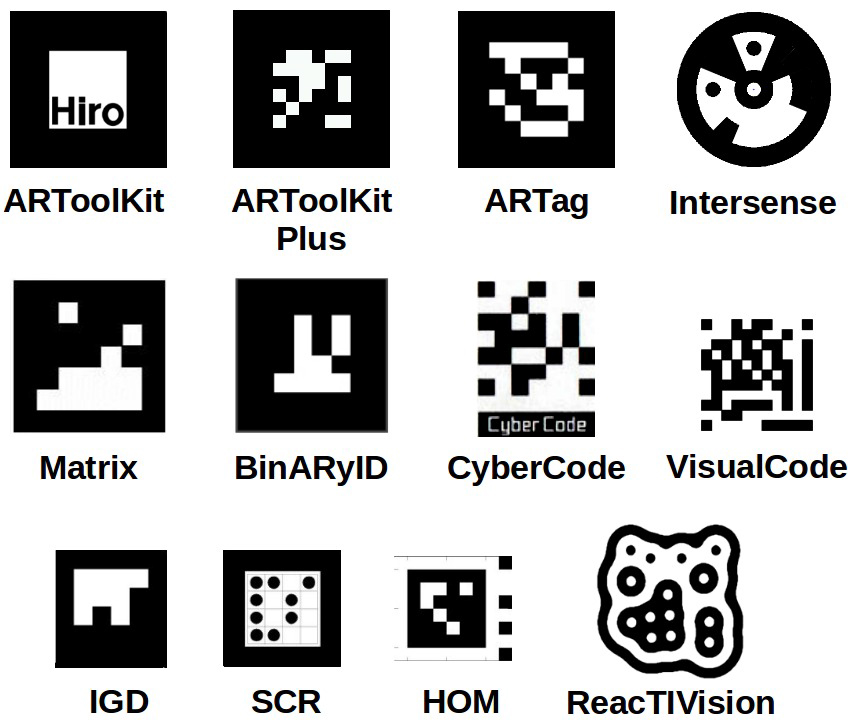
\includegraphics[width=8cm]{Bilder/BinMuster.jpg}			
	\caption{Diverse Binäre Muster die als Code für Marker Tracking verwendet werden. Quelle: \cite{article:Aruco2014}}
	\label{fig:BinMarker}
\end{figure}
